% update for ECCV'14 by Michael Stark and Mario Fritz
% updated in April 2002 by Antje Endemann
% Based on CVPR 07 and LNCS, with modifications by DAF, AZ and elle, 2008 and AA, 2010, and CC, 2011; TT, 2014

\documentclass[runningheads]{llncs}
\usepackage{graphicx}
\usepackage{amsmath,amssymb} % define this before the line numbering.
\usepackage{color}\usepackage[width=122mm,left=12mm,paperwidth=146mm,height=193mm,top=12mm,paperheight=217mm]{geometry}
\begin{document}
% \renewcommand\thelinenumber{\color[rgb]{0.2,0.5,0.8}\normalfont\sffamily\scriptsize\arabic{linenumber}\color[rgb]{0,0,0}}
% \renewcommand\makeLineNumber {\hss\thelinenumber\ \hspace{6mm} \rlap{\hskip\textwidth\ \hspace{6.5mm}\thelinenumber}}
% \linenumbers
\pagestyle{headings}
\mainmatter
\title{I know what you did, wearn and eat in the last 10 years} % Replace with your title

\titlerunning{I know what you did\dots }

\authorrunning{Dr. Bossard\dots}

\author{Dr. Lukas Bossard}
\institute{BiWi - ETH Zurich}


\maketitle

\begin{abstract}
TODO
\keywords{ETH, 10, Call me Dr., Hungry, Awesomeness, Pysome}
\end{abstract}


\section{Introduction}




This document serves as an example paper. It illustrates the format
we expect authors to follow when submitting the camera ready version to ECCV. 

\begin{figure}
\centering
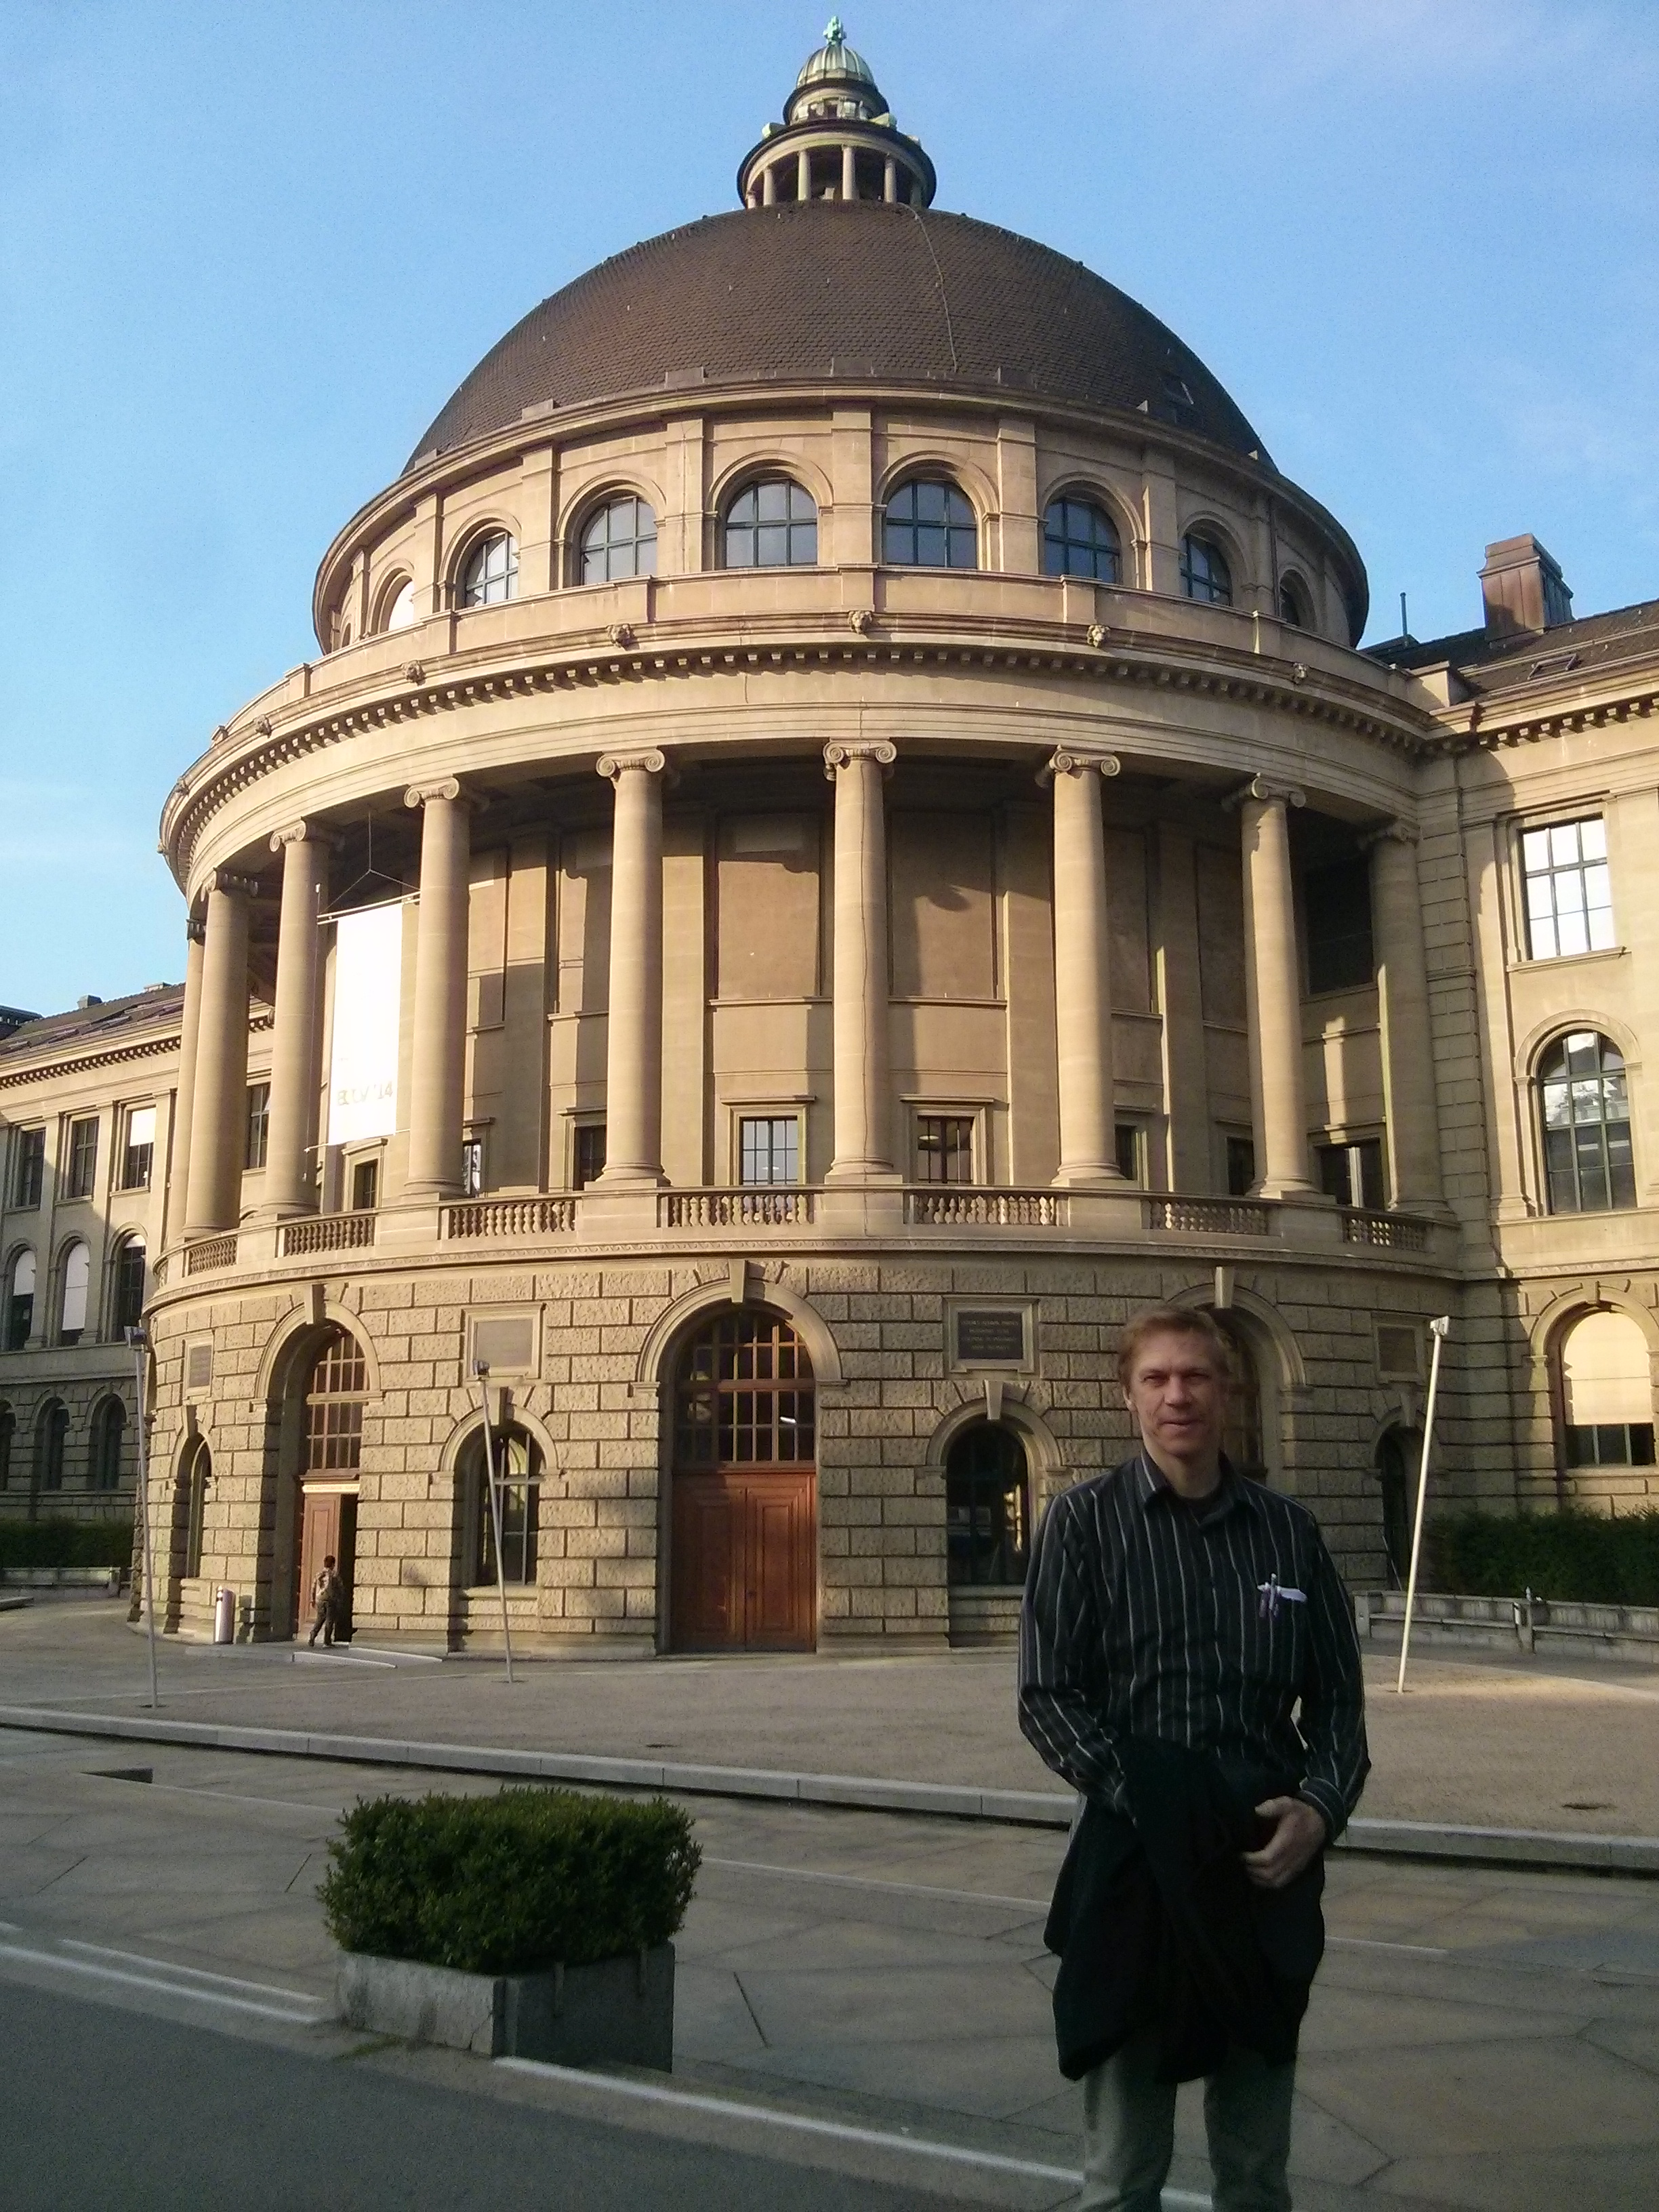
\includegraphics[height=6.5cm]{images/luc.jpg}
\caption{One kernel at $x_s$ ({\it dotted kernel}) or two kernels at
$x_i$ and $x_j$ ({\it left and right}) lead to the same summed estimate
at $x_s$. This shows a figure consisting of different types of
lines. Elements of the figure described in the caption should be set in
italics,
in parentheses, as shown in this sample caption. The last
sentence of a figure caption should generally end without a full stop}
\label{fig:example}
\end{figure}


\section{Paper formatting}


\begin{figure} \centering 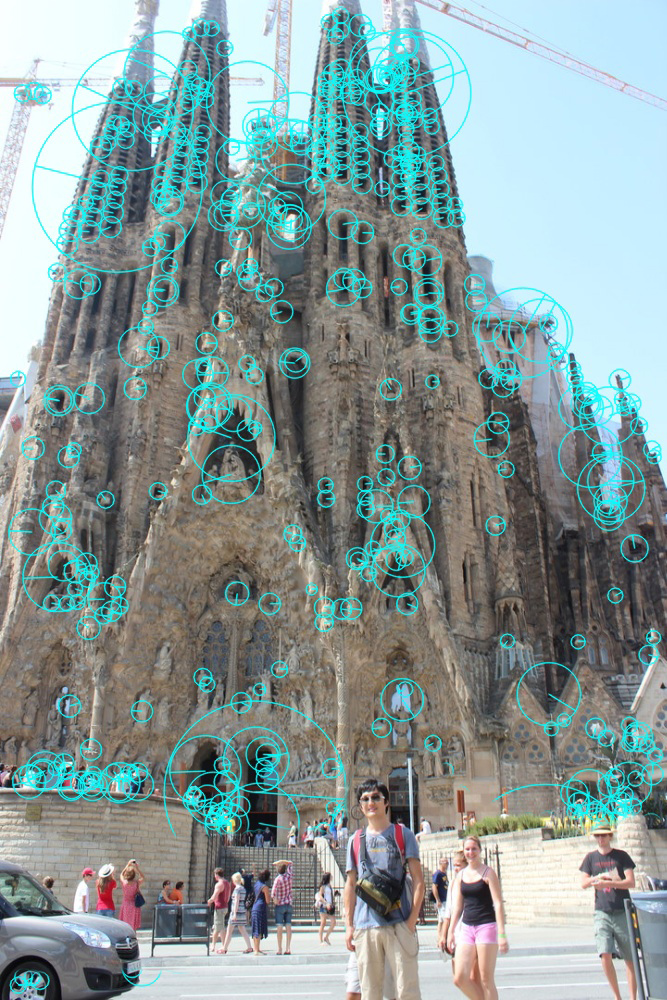
\includegraphics[height=6.5cm]{images/dengxin.jpg}
\caption{x} \label{fig:example} \end{figure}

\begin{figure} \centering 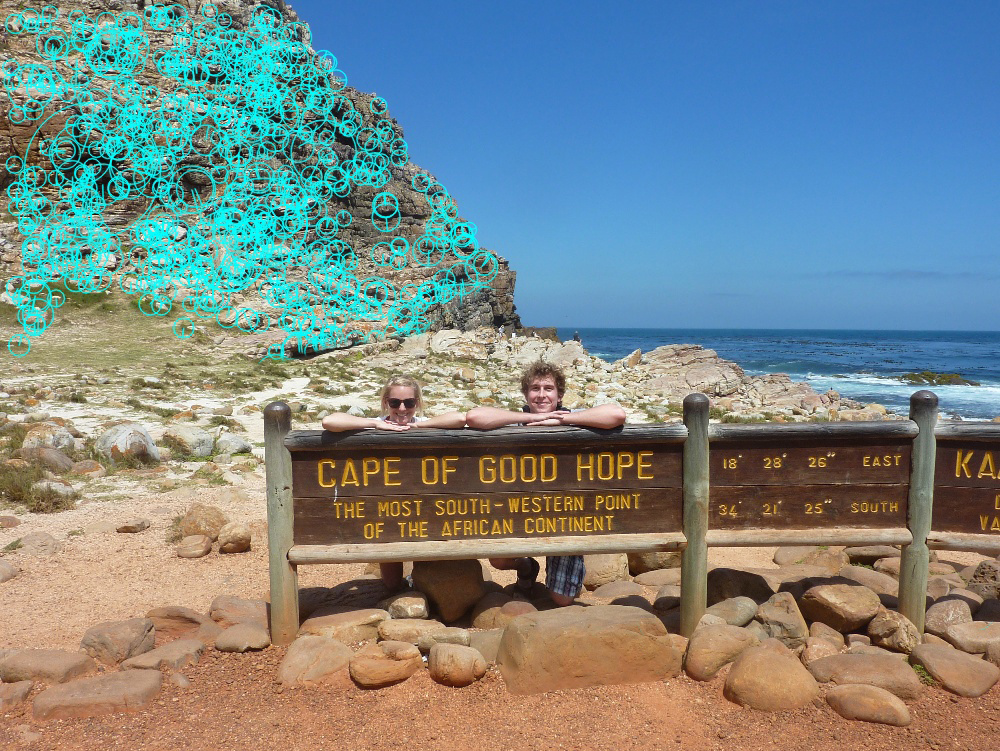
\includegraphics[height=6.5cm]{images/emmersberger.jpg}
\caption{x} \label{fig:example} \end{figure}

\begin{figure} \centering 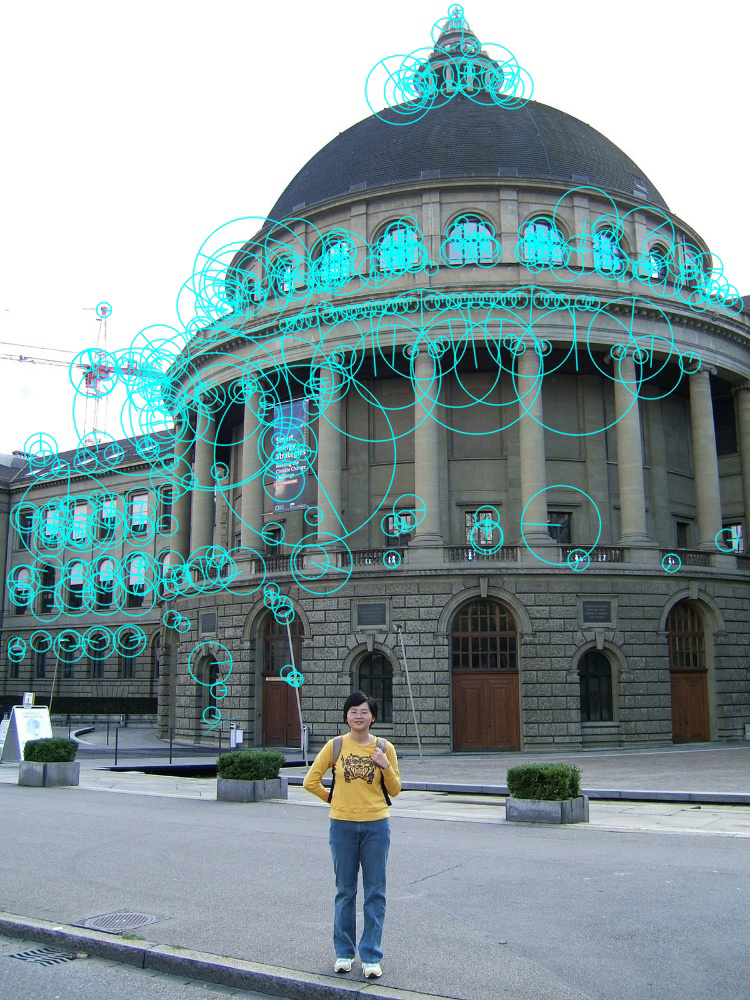
\includegraphics[height=6.5cm]{images/ETH_danfeng.jpg}
\caption{x} \label{fig:example} \end{figure}

\begin{figure} \centering 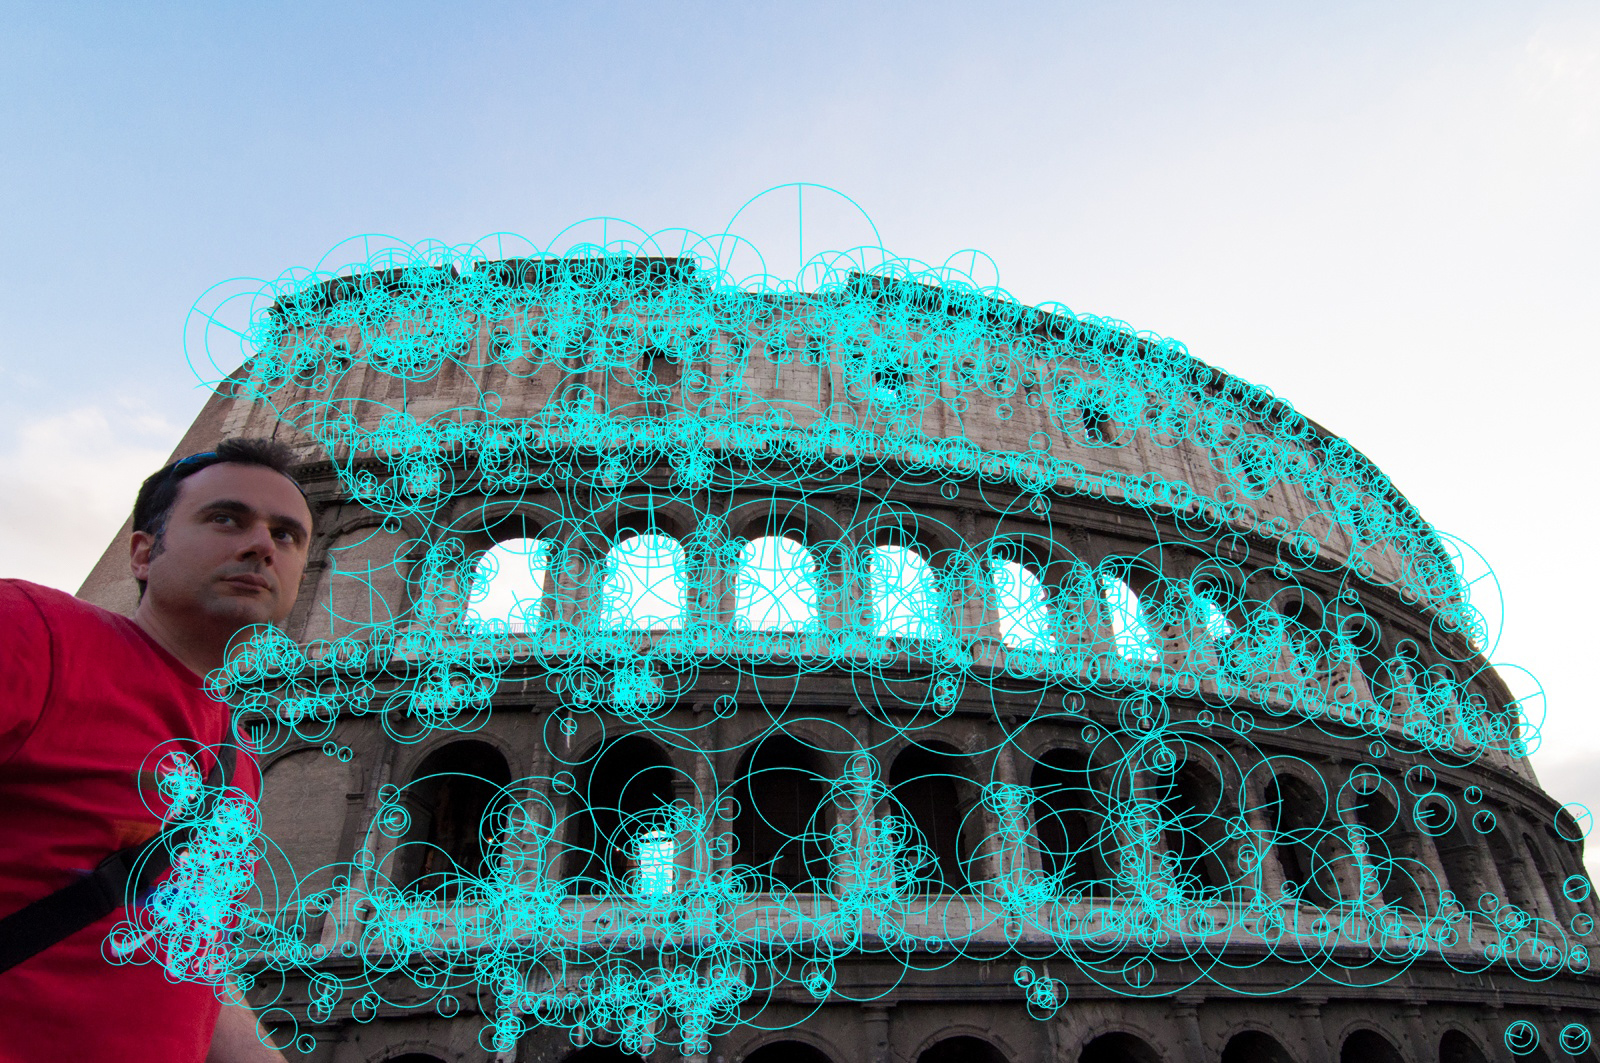
\includegraphics[height=6.5cm]{images/gabriele.jpg}
\caption{x} \label{fig:example} \end{figure}

\begin{figure} \centering 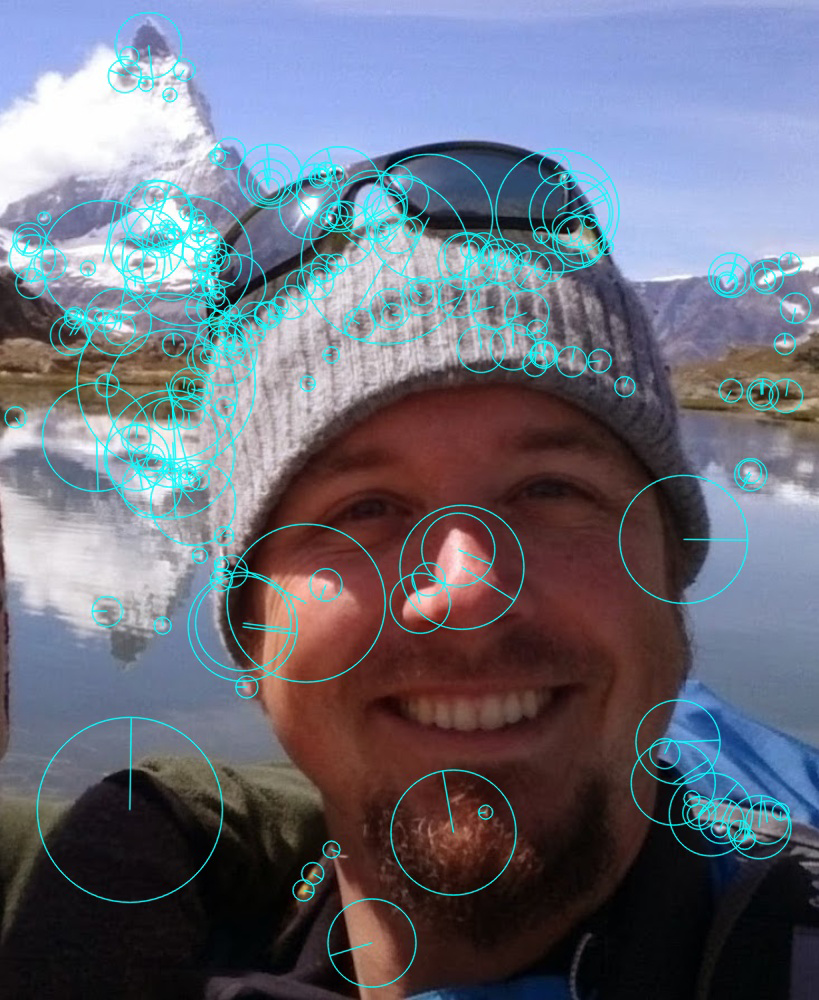
\includegraphics[height=6.5cm]{images/gass.jpg}
\caption{x} \label{fig:example} \end{figure}

\begin{figure} \centering 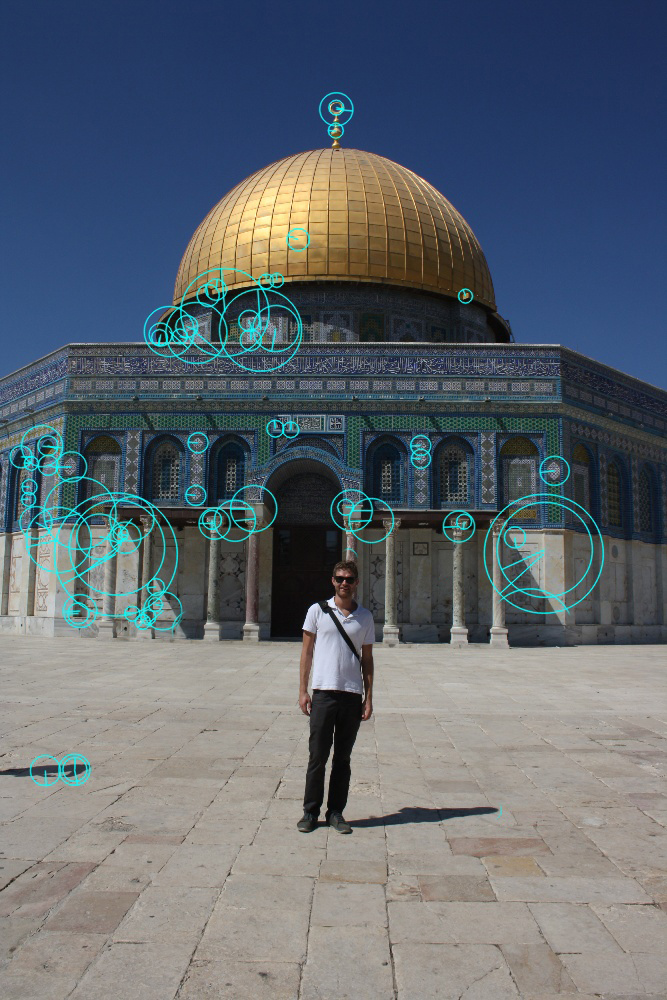
\includegraphics[height=6.5cm]{images/gygli.jpg}
\caption{x} \label{fig:example} \end{figure}

\begin{figure} \centering 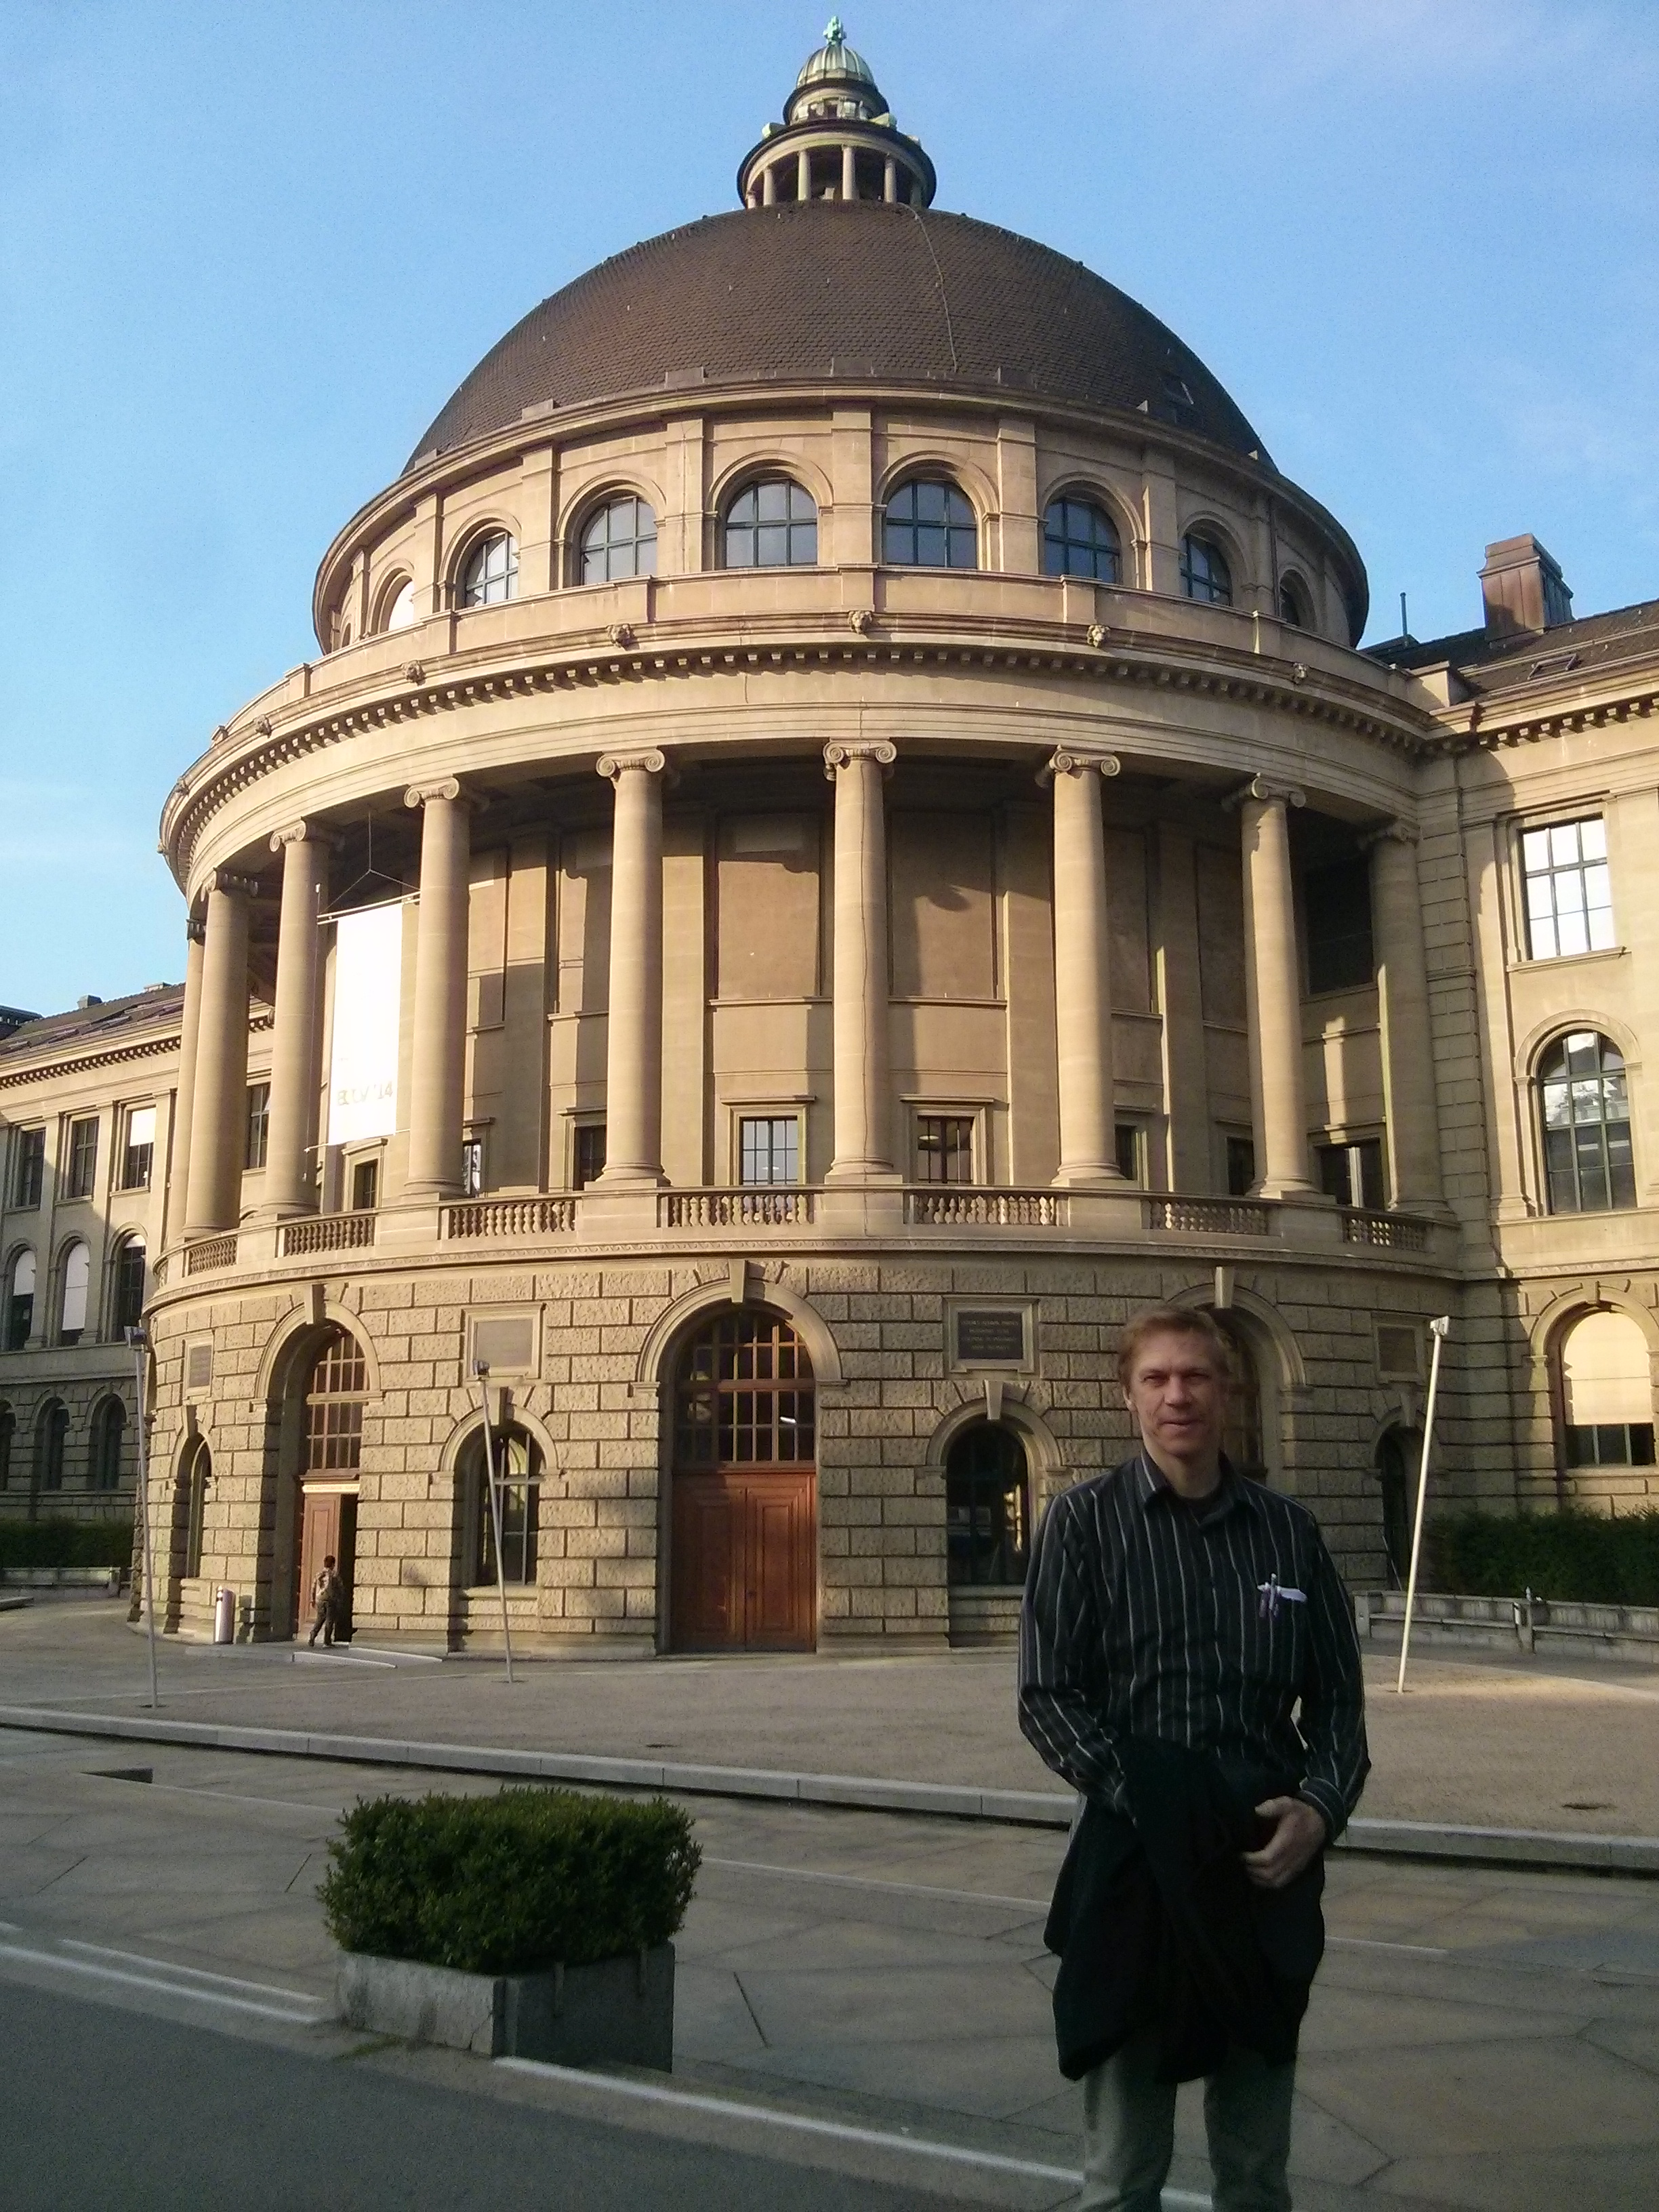
\includegraphics[height=6.5cm]{images/luc.jpg}
\caption{x} \label{fig:example} \end{figure}

\begin{figure} \centering 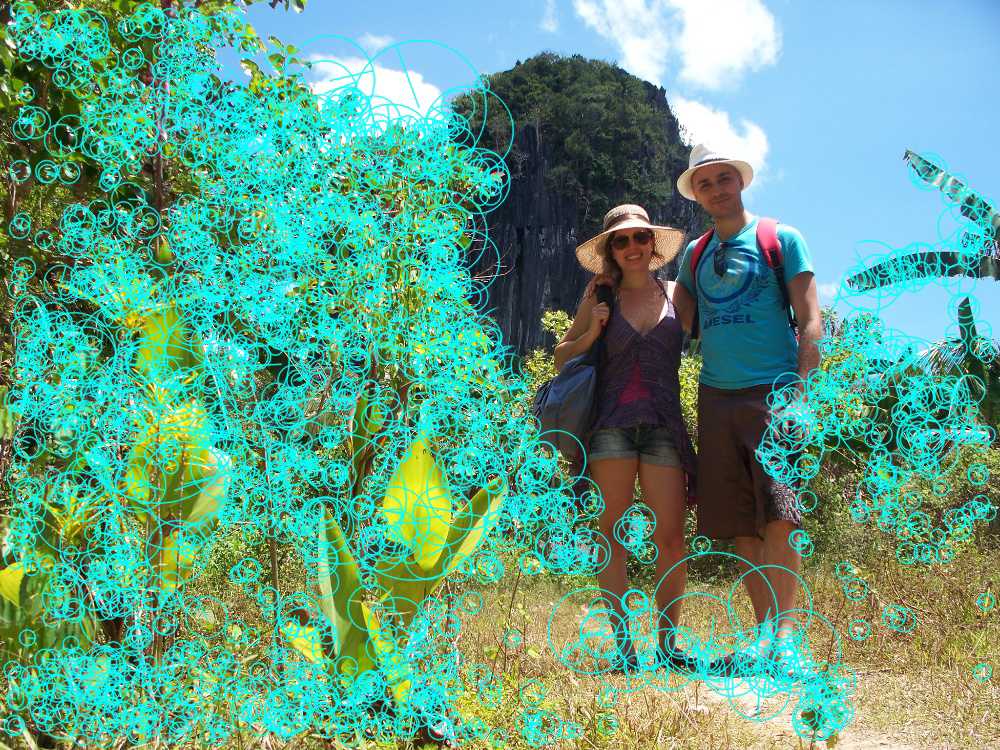
\includegraphics[height=6.5cm]{images/manen.jpg}
\caption{x} \label{fig:example} \end{figure}

\begin{figure} \centering 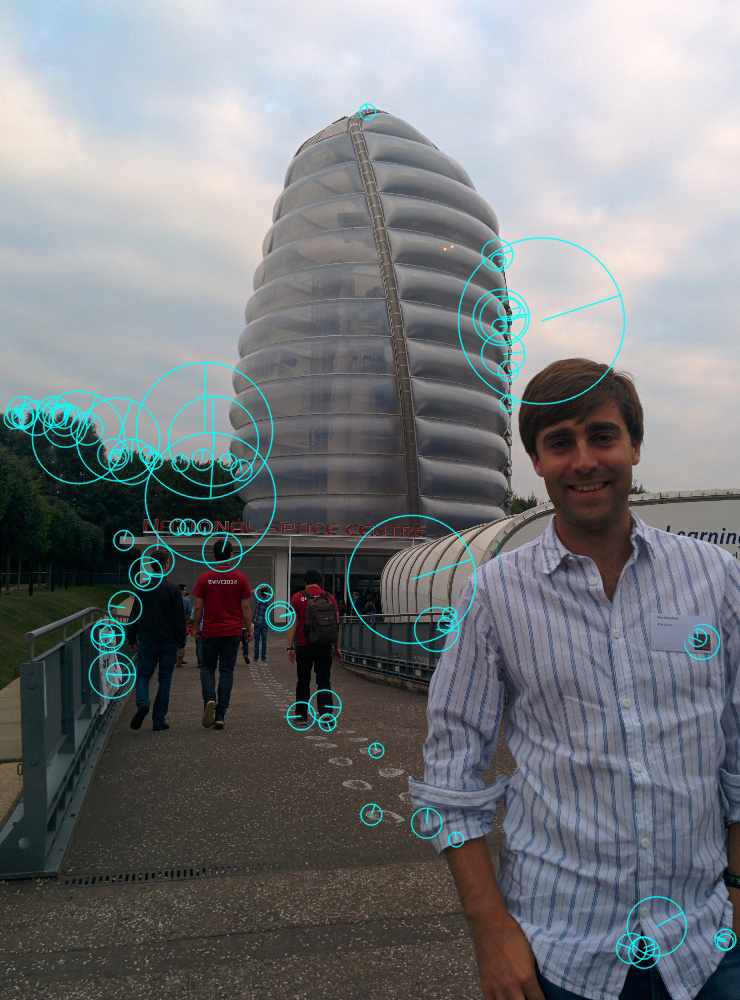
\includegraphics[height=6.5cm]{images/mansfield.jpg}
\caption{x} \label{fig:example} \end{figure}

\begin{figure} \centering 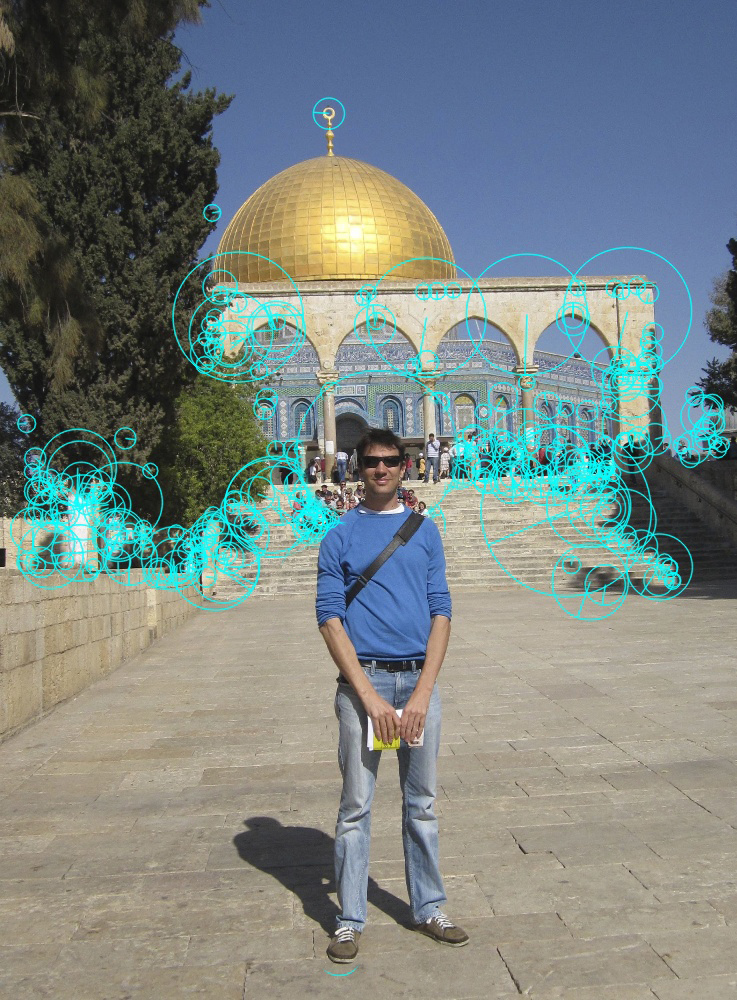
\includegraphics[height=6.5cm]{images/nater.jpg}
\caption{x} \label{fig:example} \end{figure}

\begin{figure} \centering 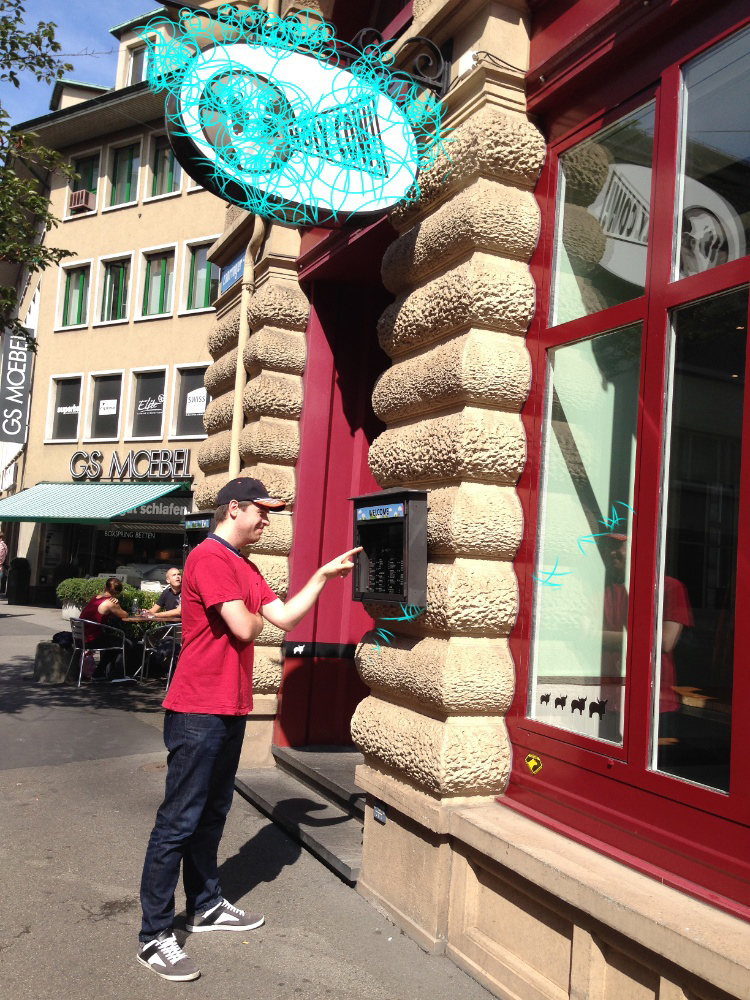
\includegraphics[height=6.5cm]{images/russ.jpg}
\caption{x} \label{fig:example} \end{figure}

\begin{figure} \centering 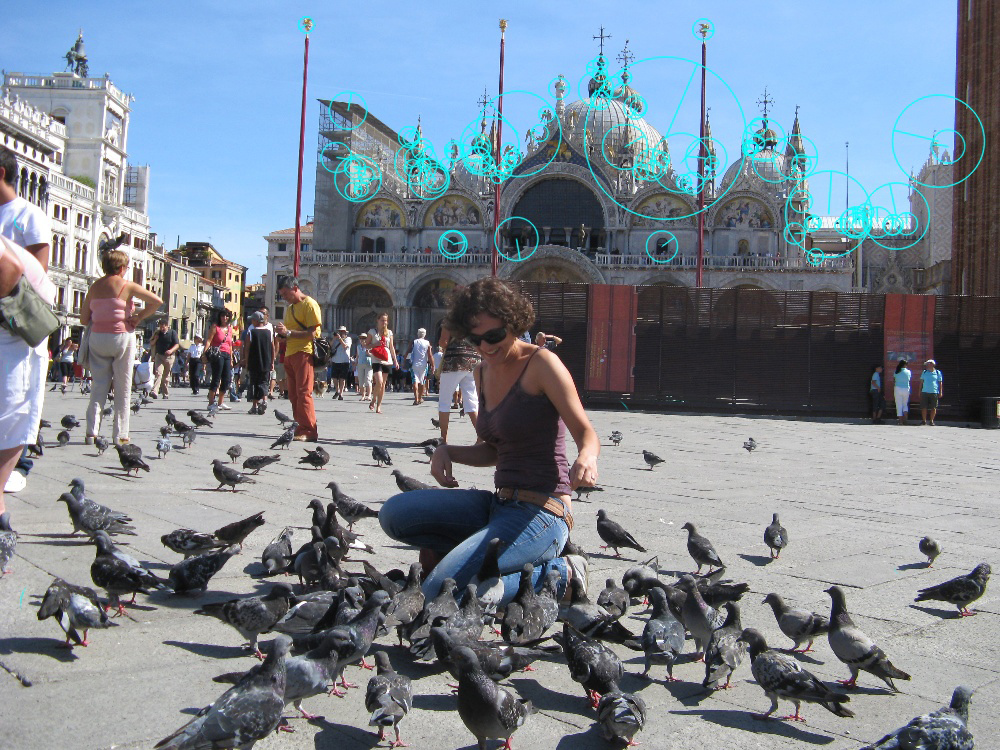
\includegraphics[height=6.5cm]{images/samei.jpg}
\caption{x} \label{fig:example} \end{figure}

\begin{figure} \centering 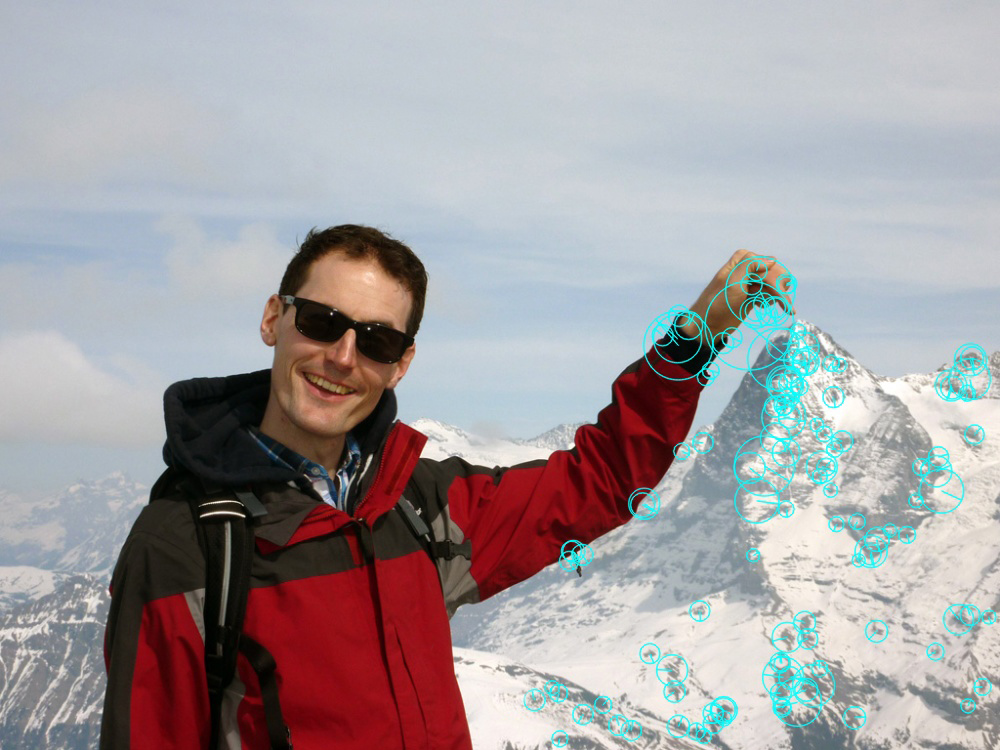
\includegraphics[height=6.5cm]{images/schneider.jpg}
\caption{x} \label{fig:example} \end{figure}

\begin{figure} \centering 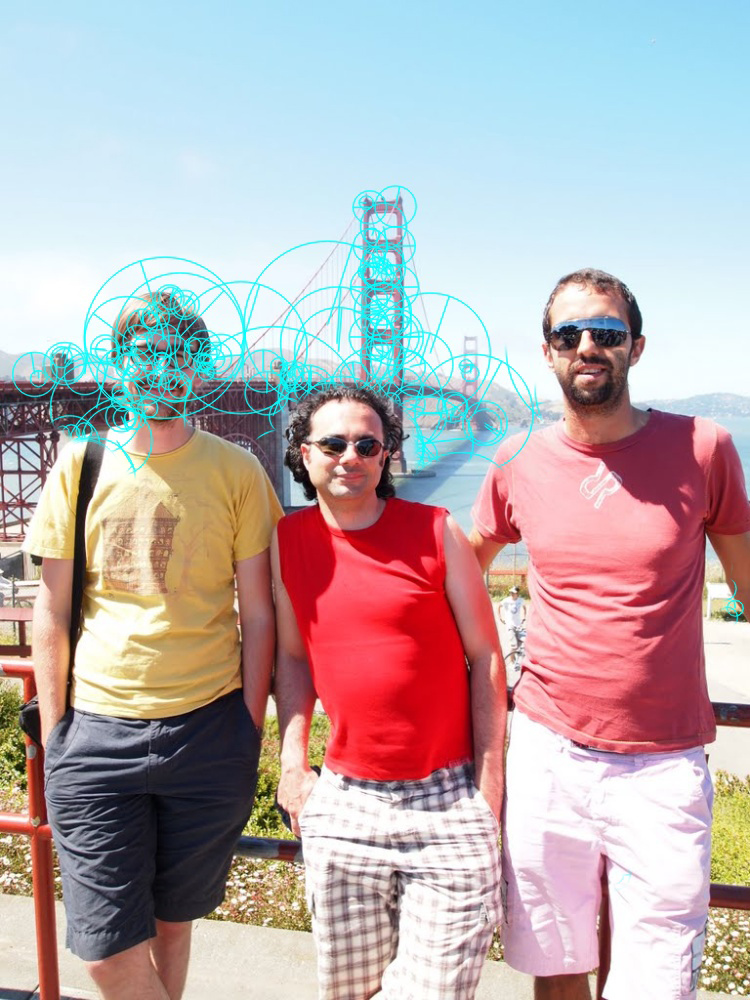
\includegraphics[height=6.5cm]{images/SF.jpg}
\caption{x} \label{fig:example} \end{figure}

\begin{figure} \centering 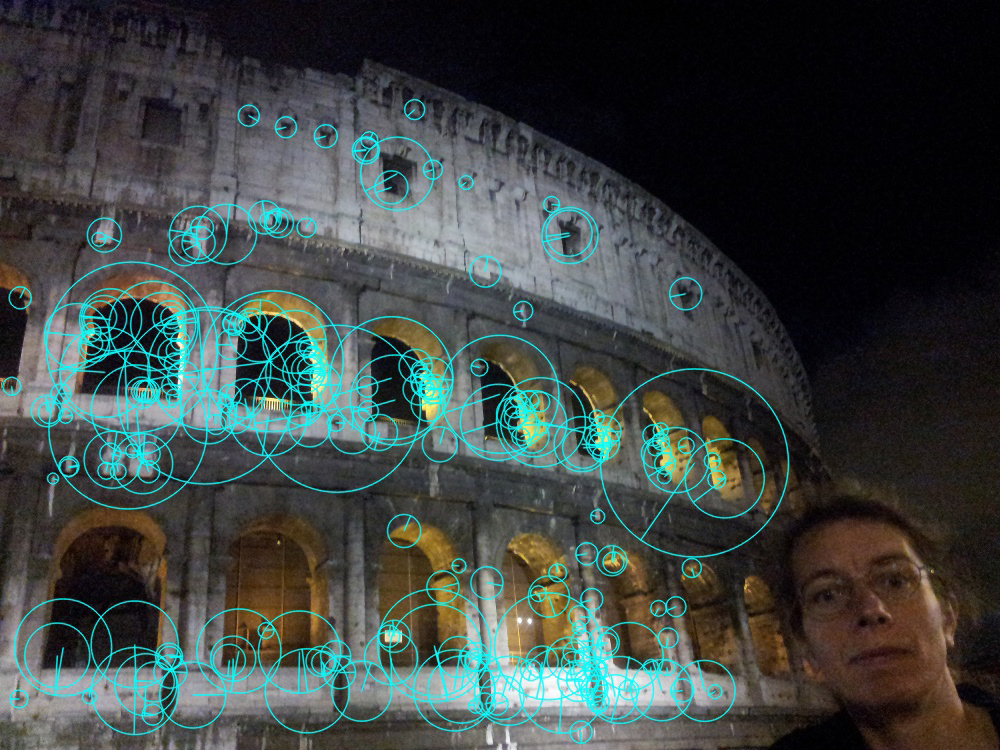
\includegraphics[height=6.5cm]{images/tanner.jpg}
\caption{x} \label{fig:example} \end{figure}

\begin{figure} \centering 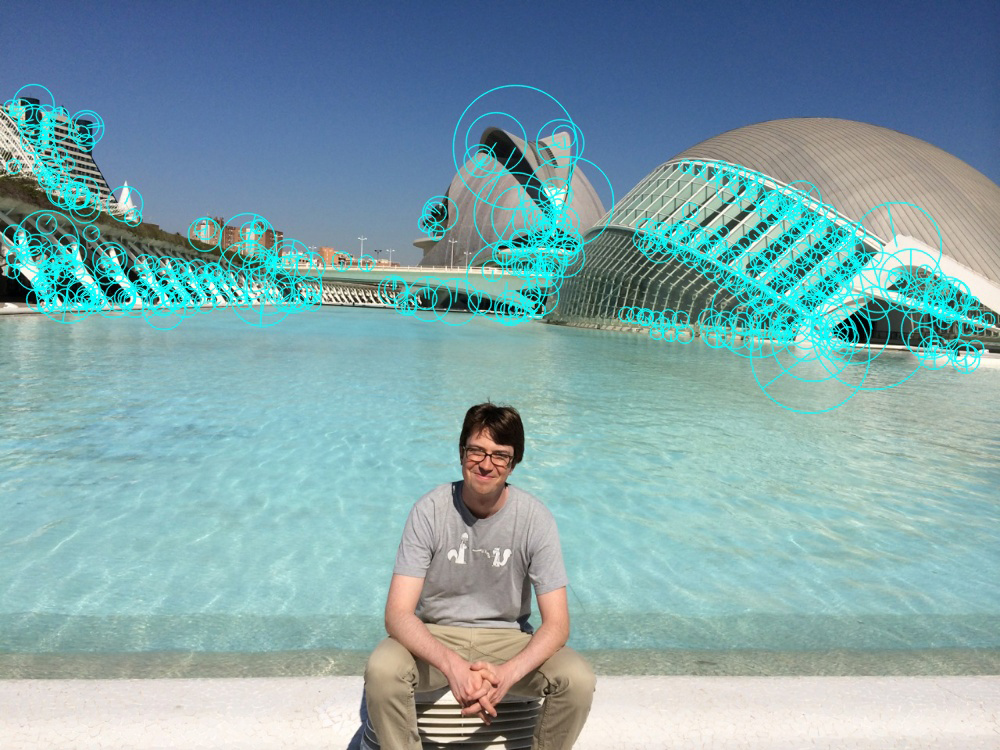
\includegraphics[height=6.5cm]{images/till2.jpg}
\caption{x} \label{fig:example} \end{figure}

\begin{figure} \centering 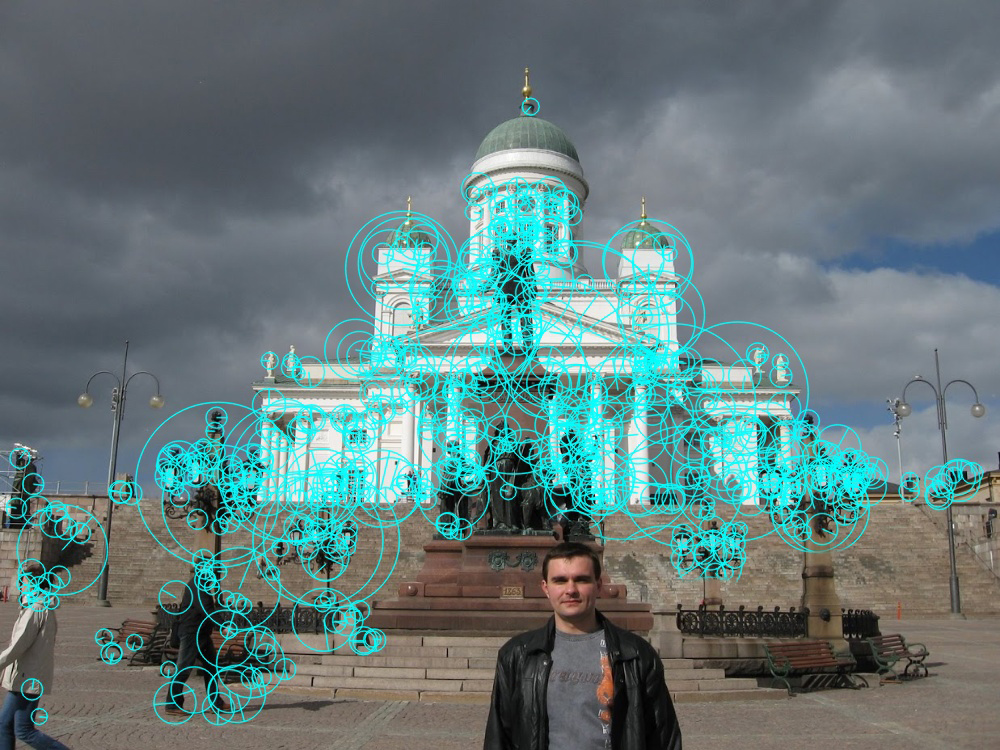
\includegraphics[height=6.5cm]{images/timofte.jpg}
\caption{x} \label{fig:example} \end{figure}

\begin{figure} \centering 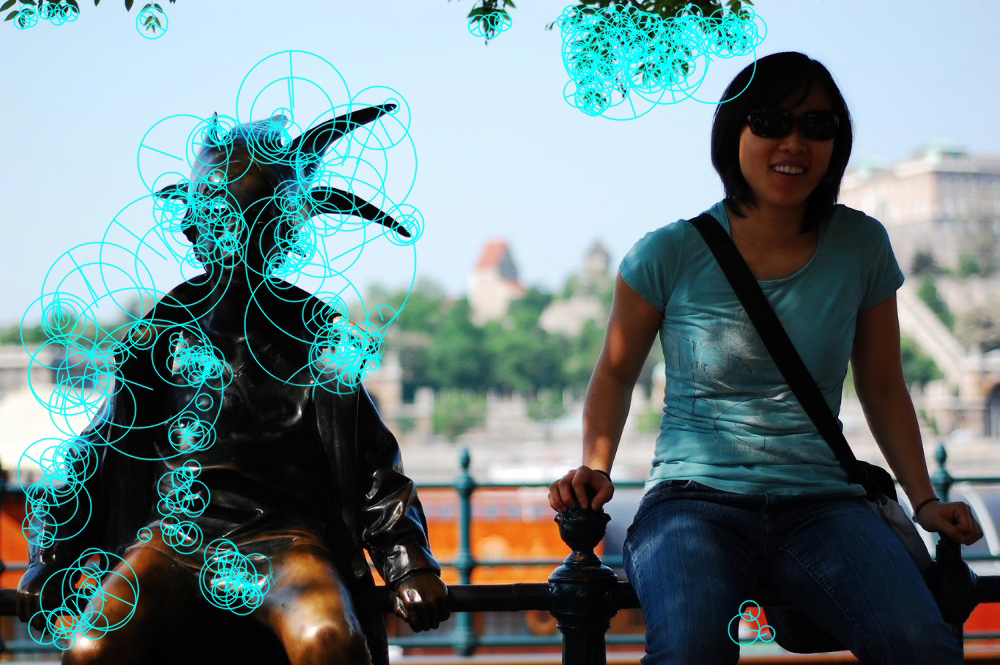
\includegraphics[height=6.5cm]{images/yao2.jpg}
\caption{x} \label{fig:example} \end{figure}


\subsection{Citations}

\section{Conclusions}

The paper ends with a conclusion. 

\par\vfill\par
Now we have reached the maximum size of the ECCV 2014 paper (excluding references).
References should start immediately after the main text, but can continue on p.15 if needed.

\clearpage

\bibliographystyle{splncs03}
\bibliography{egbib}
\end{document}
